\documentclass[a4paper,12pt]{article}

\usepackage{geometry}
\usepackage{polski}
\usepackage{amsmath}
\usepackage{makecell}
\usepackage{ragged2e}
\usepackage{graphicx}
\usepackage{xcolor}
\definecolor{MyOrange}{HTML}{D12F17}
\definecolor{MyBlue}{HTML}{00064E}
\usepackage{siunitx}
\sisetup{math-micro=\text{µ},text-micro=µ}
\usepackage{textcomp}

\graphicspath{ {./images/} }

\newcommand\crule[3][black]{\textcolor{#1}{\rule{#2}{#3}}}

\geometry{
 a4paper,
 total={170mm,257mm},
 left=20mm,
 top=20mm,
 }

\begin{document}
\title{Układy Elektroniczne - Sprawozdanie 2}
\author{Hubert Mazur \\ Piotr Moszkowicz} 
\date{\today}
\maketitle
\pagenumbering{roman}

\newpage
\begin{justify}
\tableofcontents
\newpage
\pagenumbering{arabic}

\section{Wstęp teoretyczny}
Wzmacniacz operacyjny jest aktywnym elementem elektronicznym o symetrycznym wyjściu i asymetrycznym wejściu rożnicowym. W zależności, na które wejście zostanie podane napięcie wzmacniacz może odwracać fazę napięcia wejściowego względem napięcia wejściowego, lub na wyjście przekazać napięcie o nieodwróconej fazie. Cechą charakterystyczną wzmacniaczy jest praca w pętli sprzężenia zwrotnego, która stabilizuje ich pracę, zwiększa zakres dynamiczny pracy wzmacniacza, poprawia liniowość i poszerza pasmo przenoszenia. Do celów porównawczych wzmacniaczy stosuje się kilka parametrów:

\begin{itemize}
\item Wzmocnienie różnicowe: $ k_{UR} = \frac{ \partial U_{wy}}{ \partial U_R} $ 
\item Wejściowe napięcie niezrównoważenia $ V_{OS} $, jest to napięcie przyłożone na wejściu, dla którego napięcie wyjściowe jest zerowe, dla rzeczywistych wzmacniaczy równe $ \mu V \; - \; mV $ 
\item Temperaturowy dryf wejściowego napięcia niezrównoważenia: zmiana temperatury powoduje zmianę wejściowego napięcia niezrównoważenia, zwykle rzędu $\frac {\mu V}{C} $
\item Wzmocnienie sygnału wspólnego:  niezerowa wartość napięcia na wyjściu, mimo identycznego sygnału na obu wejściach, $ k_{US} = \frac{\partial U_{Wy}}{\partial U_S}$. Właściwość opisana jest przez współczynnik tłumienia sygnału wspólnego: $ CMRR = \frac{k_{UR}}{k_{US}}$. Dla rzeczywistych wzmacniaczy równe  80 - 120 dB. 
\item $ PSRR $- odporność wzmacniacza na zmiany napięć zasilających, dla rzeczywistych wzmacniaczy.
\item Rezystancja wejściowa: $ r_R $- rezystancja różnicowa: mierzona między wejściami wzmacniacza operacyjnego, $ r_S $- rezystancja wspólna mierzona między masą a jednym z wejść.
\item Wejściowy prąd niezrównoważenia: $ I_{OS}  \; \in \; <fA,nA> $- napięcie wyjściowe zmienia się mimo braku napięcia wejściowego. 
\end{itemize}

Porównanie wzmacniaczy operacyjnych: rzeczywistego i idealnego:
\begin{center}
\begin{tabular}{ |l|c|c| }
\hline
Parametry & Idealny WO & Rzeczywisty WO \\
\hline
wzmocnienie  różnicowe:  & $\infty$ & $10^5$ \; - \; $10^7$ \\
pasmo  przenoszenia: & $0 - \infty$ & ~MHz \\
napięcie niezrównoważenia: & 0 & ~ $\mu V - mV$ \\
CMRR: & $\infty$ & ~ 80 - 120 dB \\
PSRR: & $\infty$ & ~ 50 - 120 dB \\
rezystancja wejściowa: & $\infty$ & ~ M $\Omega$ \\
rezystancja wyjściowa: & 0 & ~ 10 - 1000 $\Omega$ \\
$I_{OS}$ & 0 & ~ fA - nA \\
\hline
\end{tabular}
\end{center}

\subsection{Slew rate \label{sr}}

Slew rate (szybkość narastania) - jest to szybkość zmiany napięcia na jednostkę czasu. Zwykle podawana w $\frac{V}{\si{\micro s}}$.

\newpage

\section{Pomiary i wyniki}

\subsection{Wtórnik napięciowy}

\subsubsection{Schemat wtórnika napięciowego}

\begin{figure}[h]
\centering
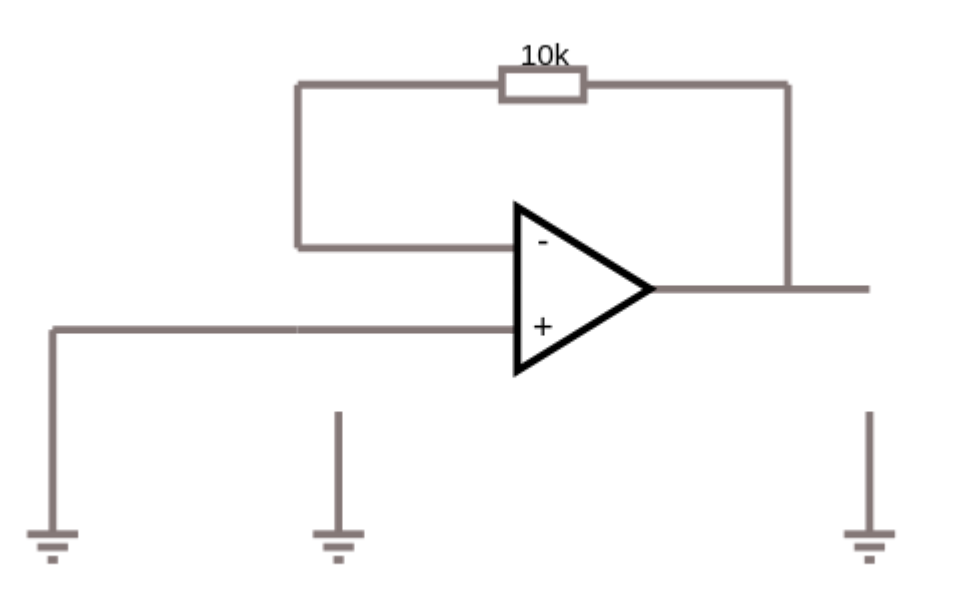
\includegraphics[width=10cm, height=6cm]{wn}
\caption{Schemat wtórnika napięciowego}
\end{figure}

\subsubsection{Zależność $U_{out}$ od $U_{in}$, wzmocnienie i napięcie zrównoważenia dla zerowej częstotliwości}

\begin{figure}[h]
\centering
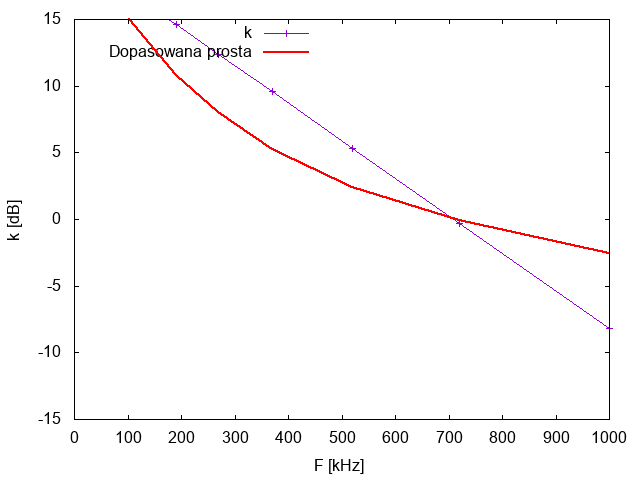
\includegraphics[width=7.5cm, height=6cm]{plot_wtornik_napieciowy}
\caption{Zależność $U_{out}$ od $U_{in}$}
\end{figure}

\paragraph{Wzmocnienie = 0.98123171}

\paragraph{Napięcie niezrównoważenia = 0V}

\paragraph{Zgodnie z teorią współczynnik wzmocnienia jest w okolicy jedynki, co również ukazuje wykres w postaci funkcji liniowej.}

\newpage

\subsubsection{Odpowiedź na skok napięcia dla sygnału małego  o wartości 100mV}

\begin{figure}[h]
\centering
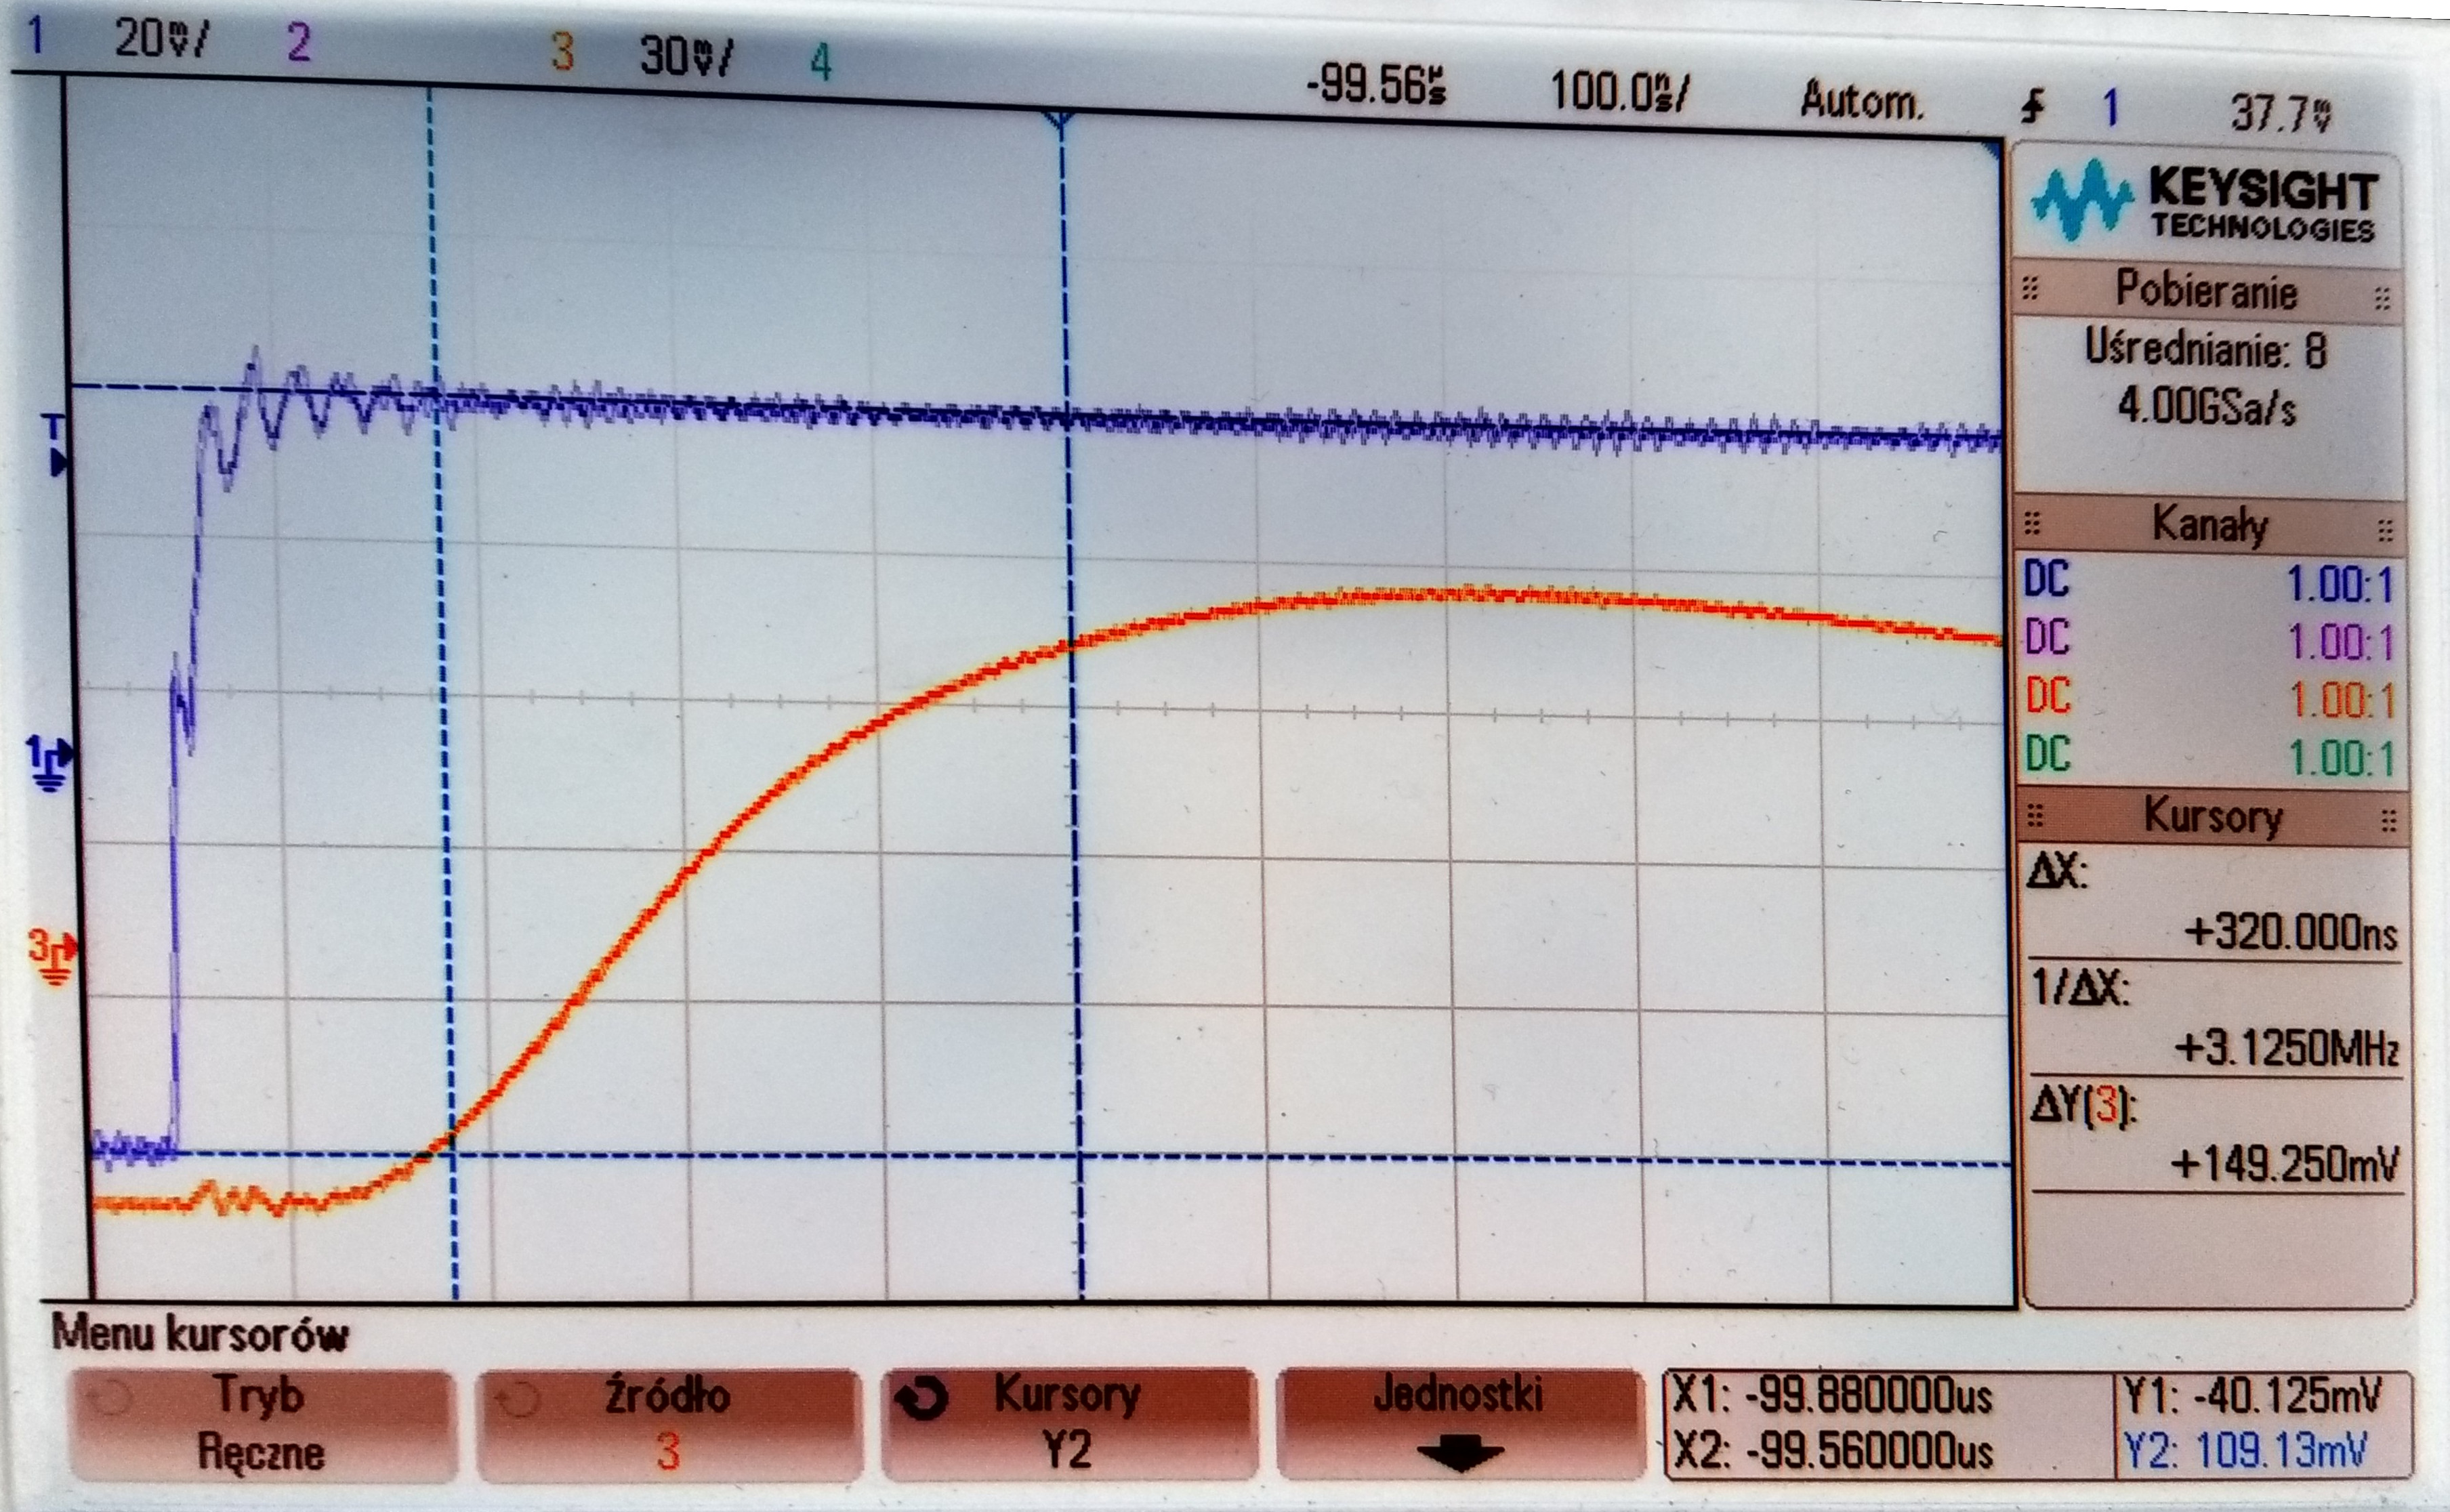
\includegraphics[width=10cm, height=7cm]{1b_amplituda_wejscia}
\caption{Amplituda odpowiedzi na sygnał mały o wartości 100mV}
\begin{tabular}{cl}
\crule[MyOrange]{1cm}{0.4cm}  & Sygnał wejścia \\
\crule[MyBlue]{1cm}{0.4cm}   & Sygnał wyjścia
\end{tabular}
\end{figure}

\paragraph{Amplituda odpowiedzi na sygnał mały o wartości 100mV wynosi: $125.25 mV$}

\subsubsection{Czas narastania odpowiedzi na skok napięcia dla sygnału małego o wartości 100mV}

\begin{figure}[h]
\centering
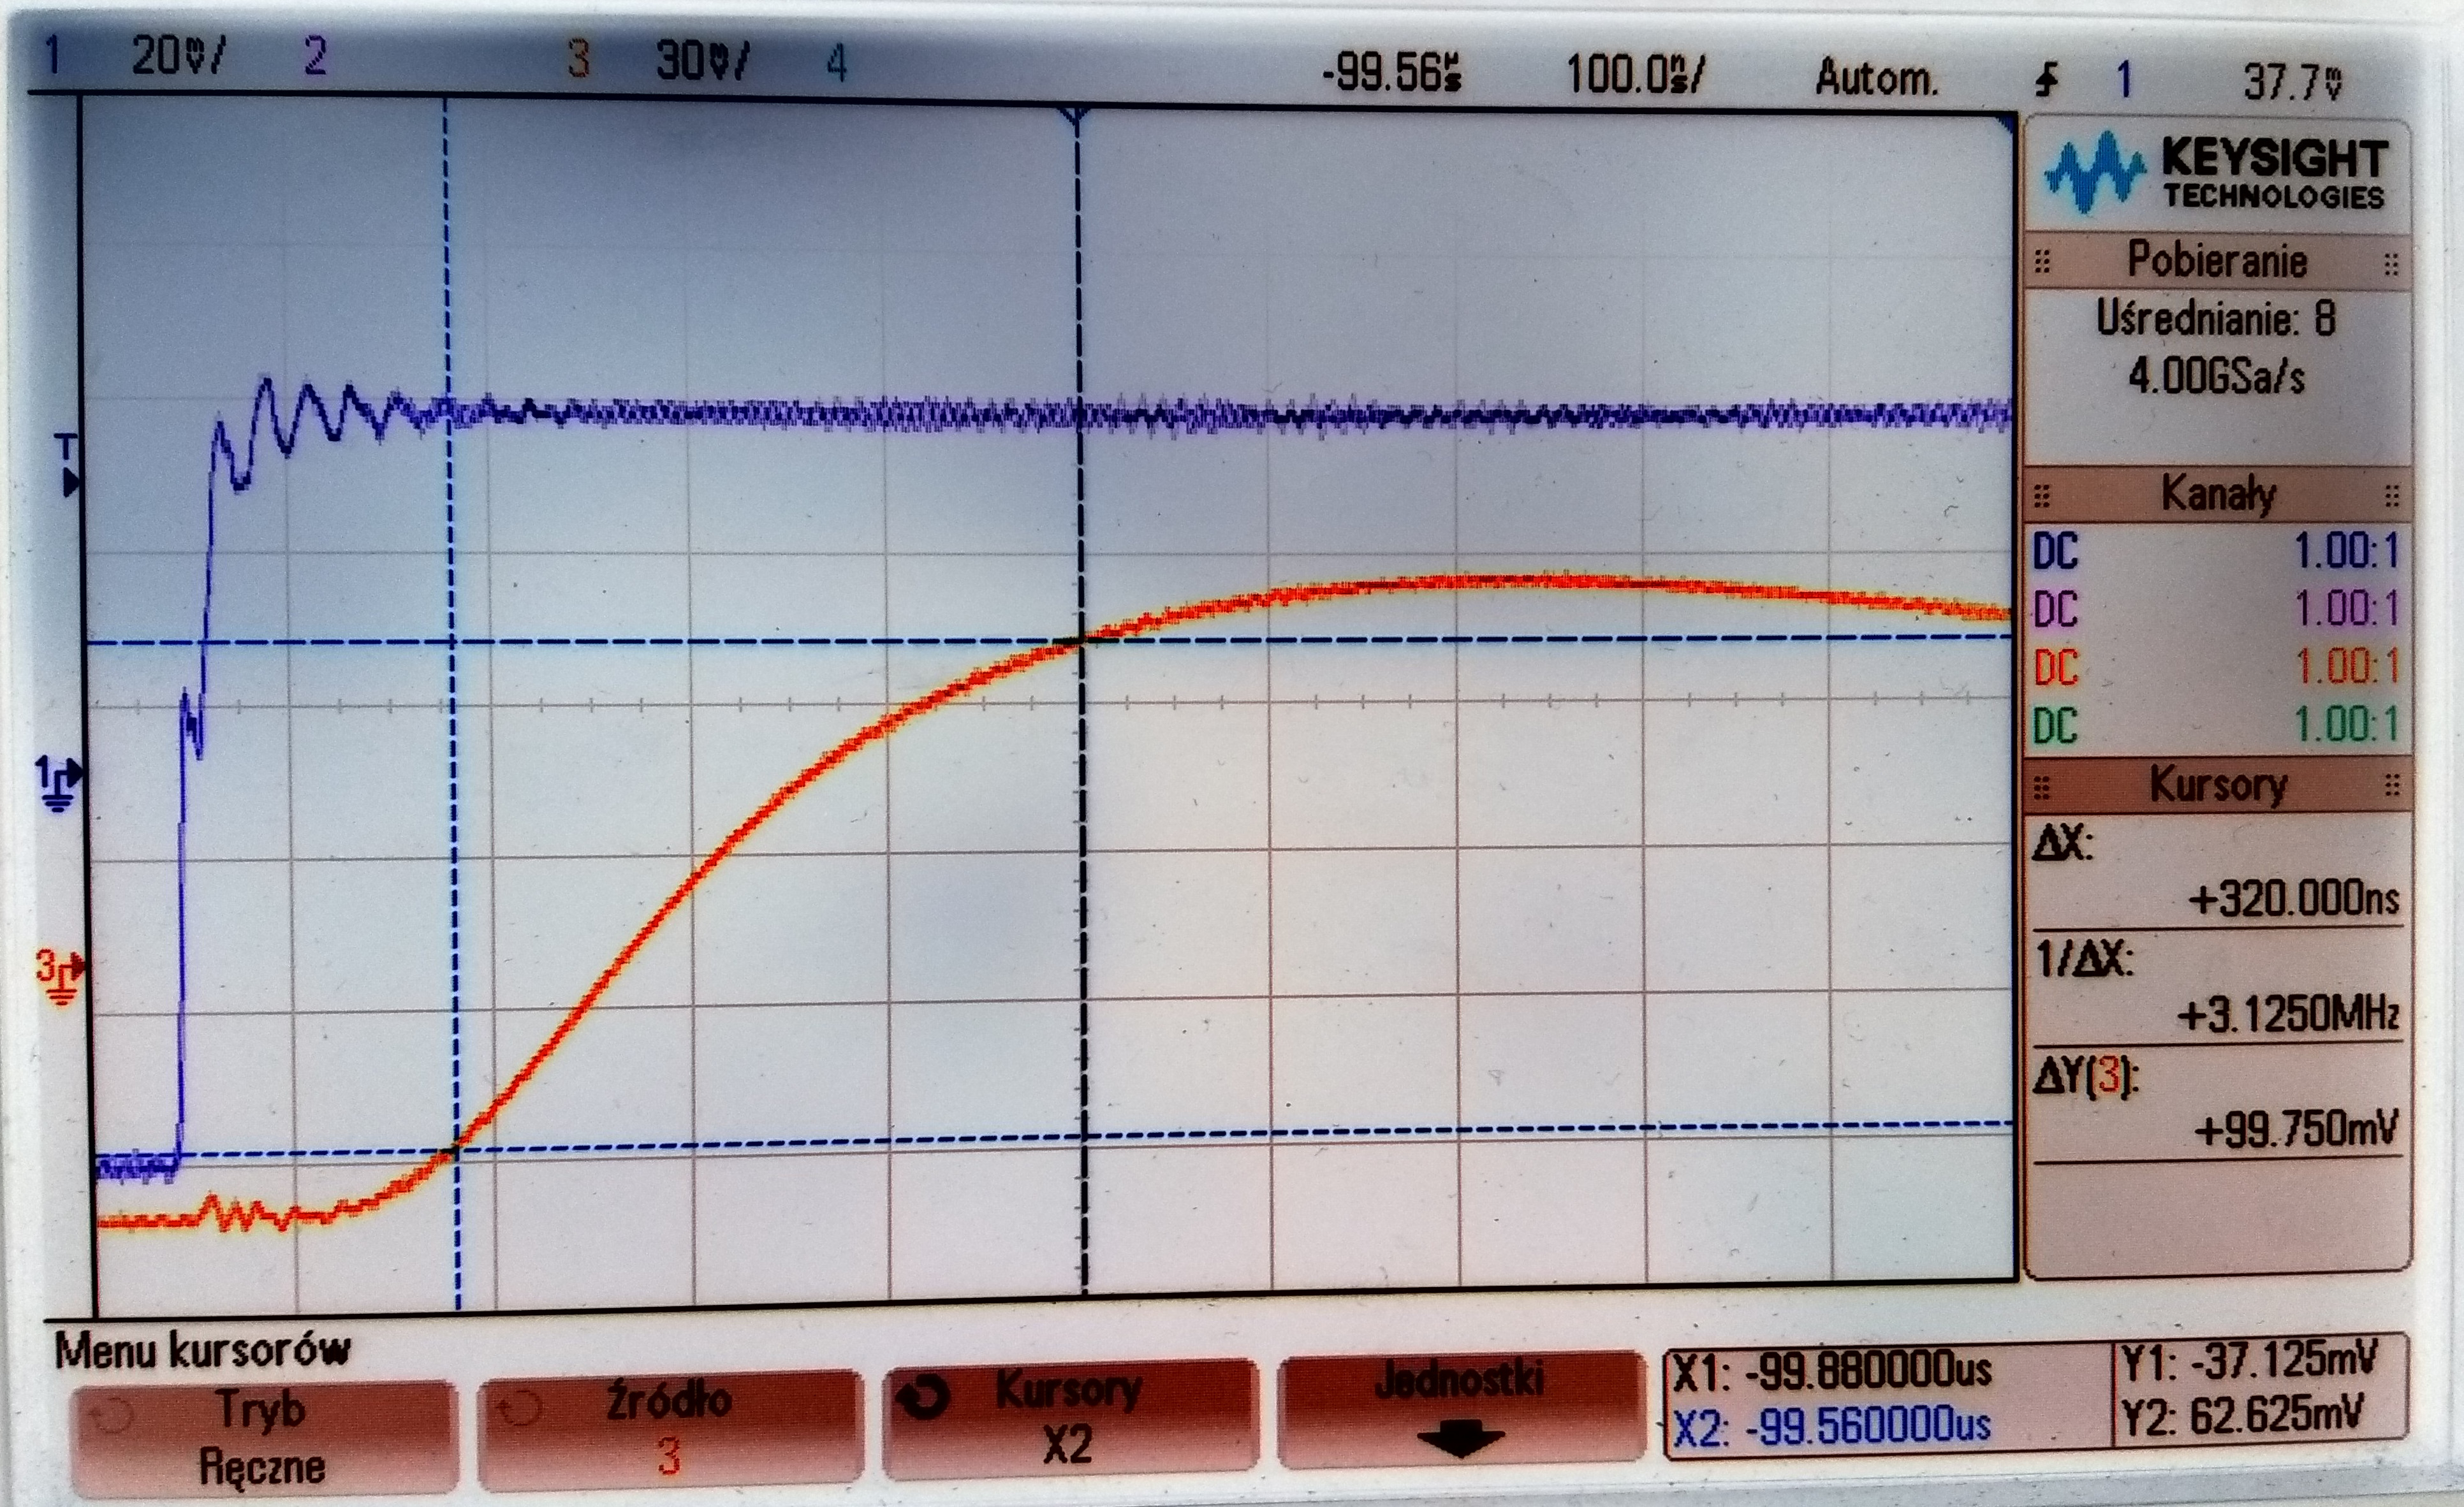
\includegraphics[width=10cm, height=7cm]{1b_czas_narastania}
\caption{Czas narastania odpowiedzi na sygnał mały o wartości 100mV}
\begin{tabular}{cl}
\crule[MyOrange]{1cm}{0.4cm}  & Sygnał wejścia \\
\crule[MyBlue]{1cm}{0.4cm}   & Sygnał wyjścia
\end{tabular}
\end{figure}

\paragraph{Czas narastania odpowiedzi na sygnały mały o wartości 100mV wynosi: $320 \si{\nano s}$}

\newpage

\subsubsection{Odpowiedź na skok napięcia dla sygnału dużego o wartości 5V oraz czas jej narastania}

\begin{figure}[h]
\centering
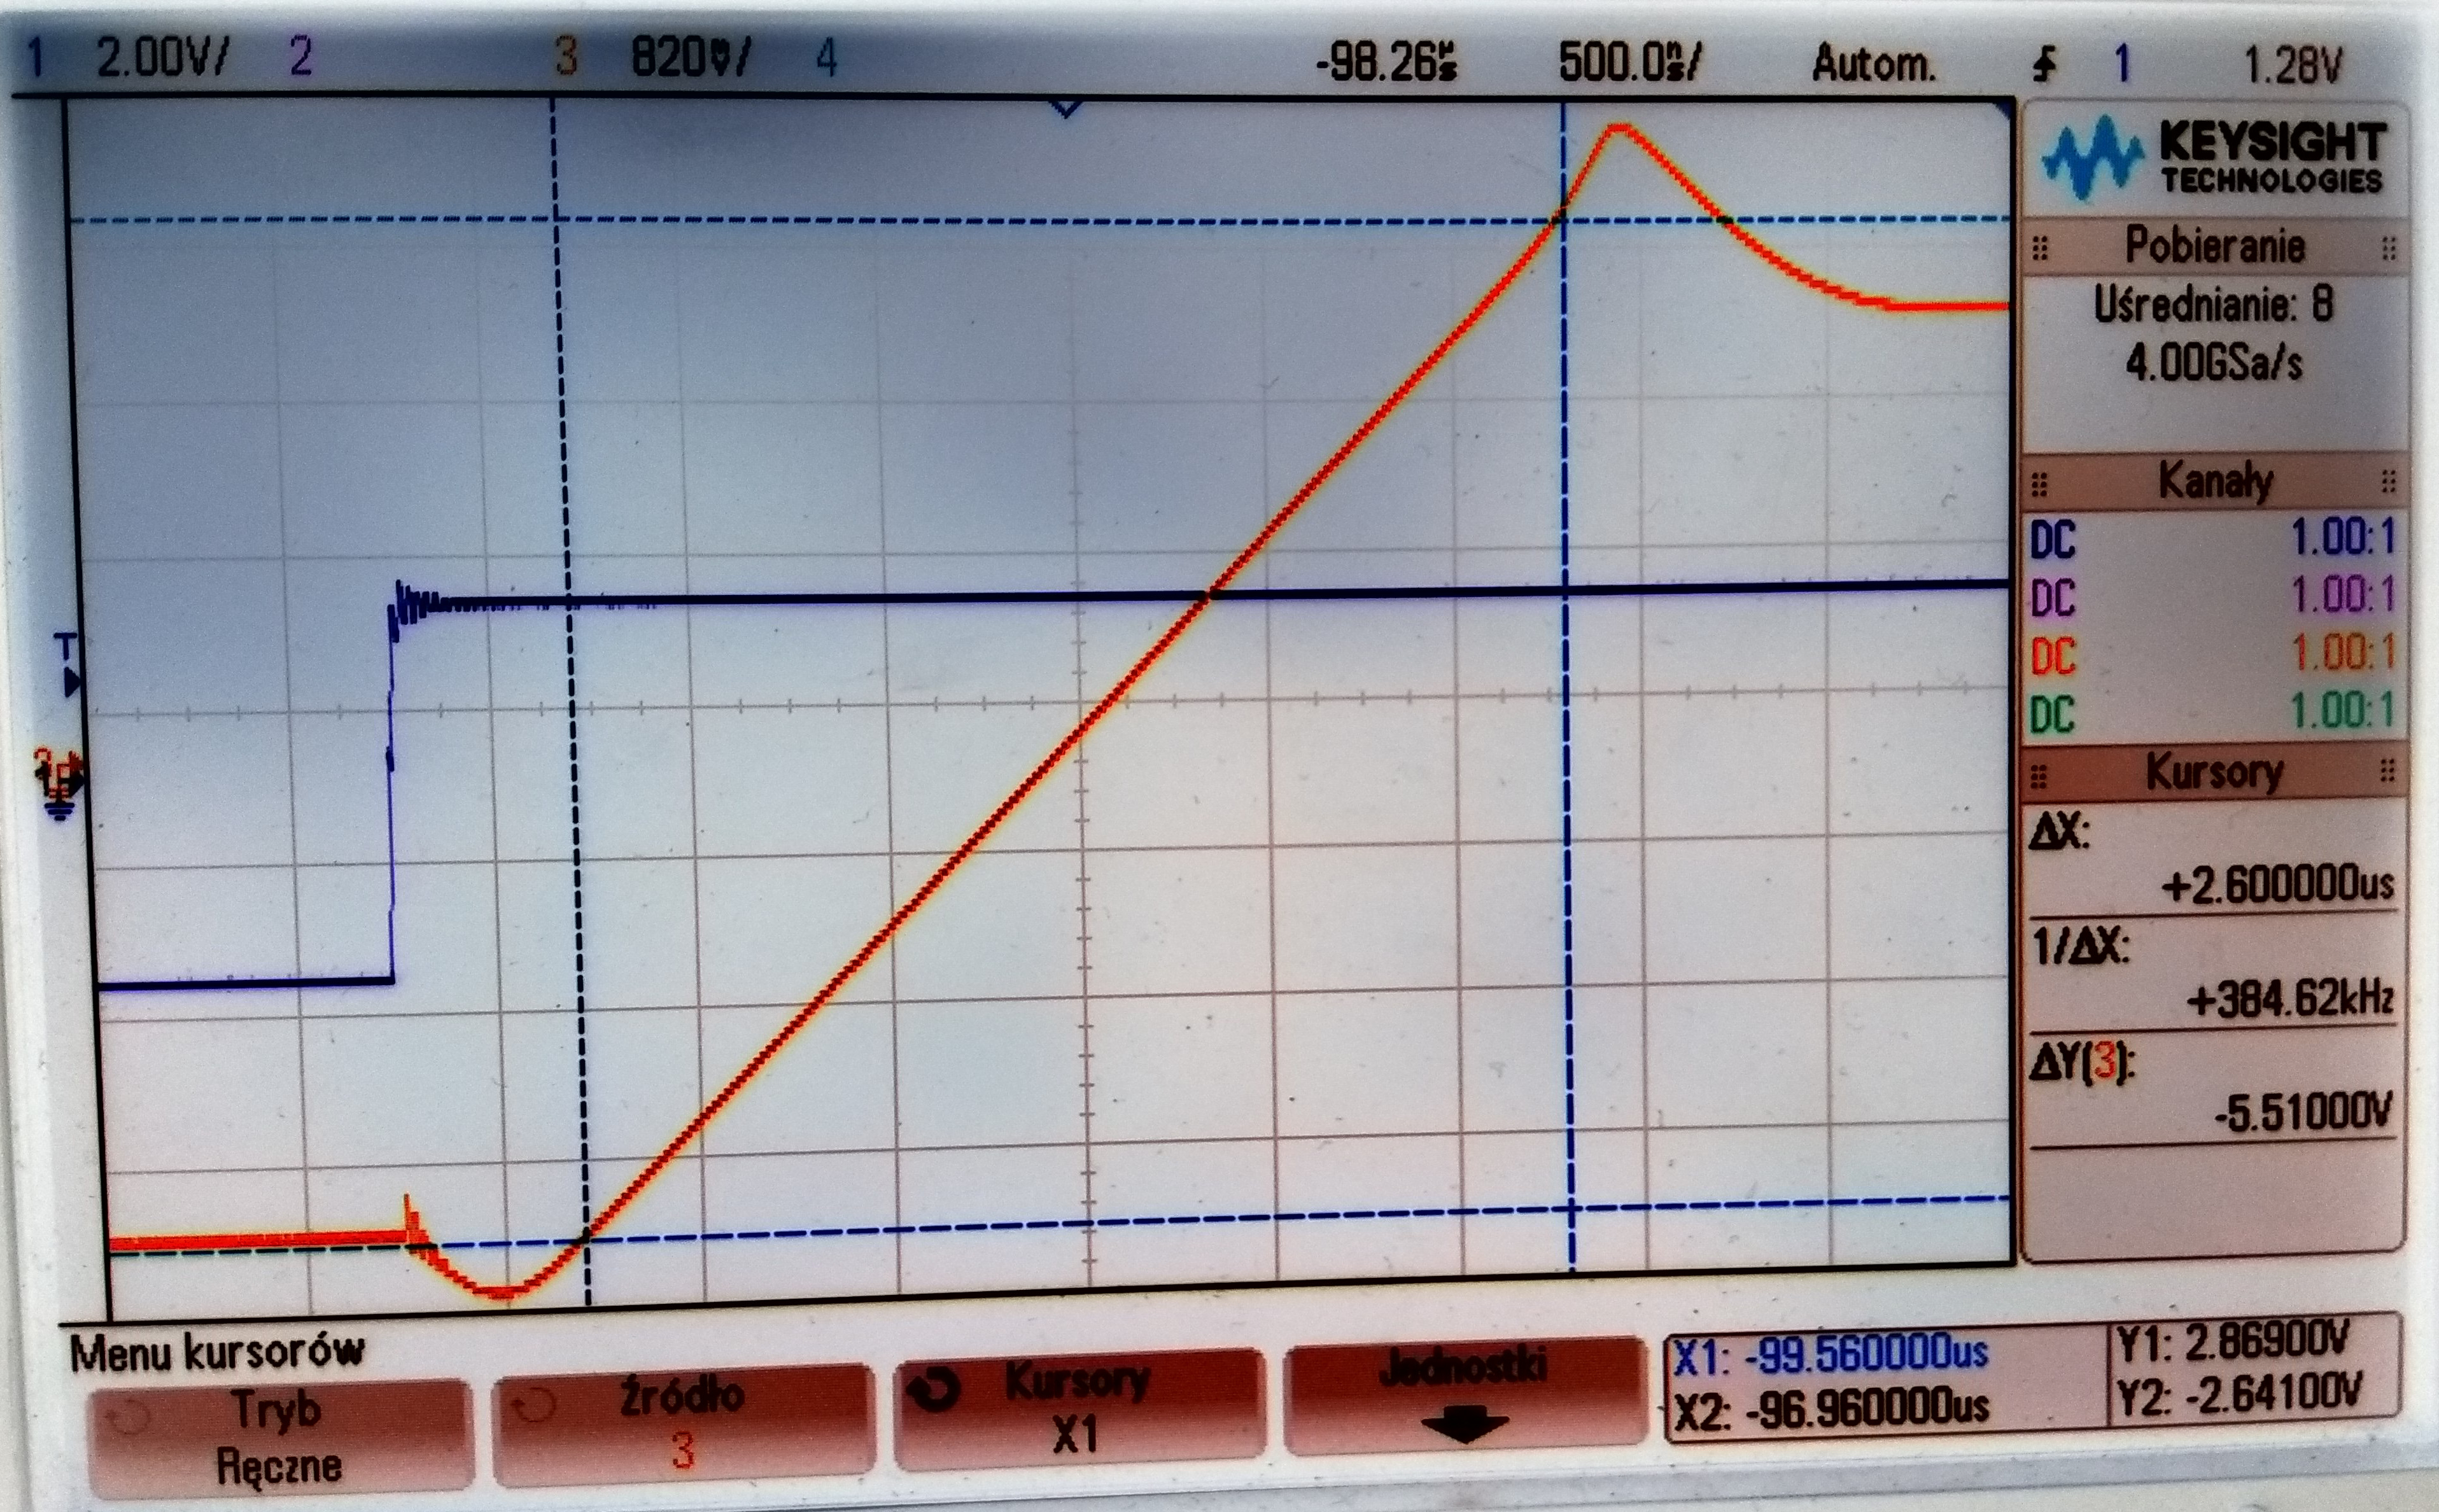
\includegraphics[width=10cm, height=7cm]{1c}
\caption{Amplituda oraz czas narastania odpowiedzi na sygnał duży o wartości 5V}
\begin{tabular}{cl}
\crule[MyOrange]{1cm}{0.4cm}  & Sygnał wejścia \\
\crule[MyBlue]{1cm}{0.4cm}   & Sygnał wyjścia
\end{tabular}
\end{figure}

\paragraph{Amplituda wyjścia: $5.51 V$ }
\paragraph{Slew rate (pkt. \ref{sr}): $2.135658915 \frac{V}{\si{\micro s}}$}
\paragraph{Czas narastania: $2.58 \si{\micro s}$}

\subsubsection{Amplitudowa charakterystyka częstotliwościowa}

\begin{center}
\begin{tabular}{ |p{3cm}|p{3cm}|p{3cm}|p{3cm}|p{3cm}| }
\hline
\makecell{Częstotliwość \\ $f$ [kHZ]} & \makecell{Wzmocnienie \\ $k$ [-]} & \makecell{Wzmocnienie \\ $k$ [dB]} & \makecell{Amplituda \\ wejścia [mV]} & \makecell{Amplituda \\ wyjścia [mV]} \\
\hline
1 & 1.003781195 & 0.032781104 & 99.175 & 99.55 \\
1.4 & 1.003781195 & 0.032781104 & 99.175 & 99.55 \\
1.9 & 1.003781195 & 0.032781104 & 99.175 & 99.55 \\
2.70 & 1.015376859 & 0.132545228 & 99.175 & 100.7 \\
3.7 & 1.015376859 & 0.132545228 & 99.175 & 100.7 \\
5.2 & 1.015376859 & 0.132545228 & 99.175 & 100.7 \\
7.2 & 1.015376859 & 0.132545228 & 99.175 & 100.7 \\
10 & 1.015376859 & 0.132545228 & 99.175 & 100.7 \\
14 & 1.015376859 & 0.132545228 & 99.175 & 100.7 \\
19 & 1.015376859 & 0.132545228 & 99.175 & 100.7 \\
27 & 1.028485001 & 0.243959252 & 99.175 & 102 \\
37 & 1.028485001 & 0.243959252 & 99.175 & 102 \\
52 & 1.028485001 & 0.243959252 & 99.175 & 102 \\
72 & 1.028485001 & 0.243959252 & 99.175 & 102 \\
100 & 1.043282462 & 0.368038134 & 99.925 & 104.25 \\
140 & 1.074626866 & 0.625153875 & 100.5 & 108 \\
190 & 1.121144279 & 0.9932301 & 100.5 & 112.675 \\
270 & 1.223476298 & 1.751911206 & 99.675 & 121.95 \\
370 & 1.313769752 & 2.370385169 & 99.675 & 130.95 \\
520 & 1.346315011 & 2.582933762 & 101.425 & 136.55 \\
720 & 1.186046512 & 1.48203441 & 102.125 & 121.125 \\
1000 & 0.928819444 & -0.641374028 & 100.8 & 93.625 \\
1400 & 0.672504378 & -3.446097678 & 99.925 & 67.2 \\
1900 & 0.501760563 & -5.990069514 & 99.4 & 49.875 \\
2700 & 0.33273703 & -9.557977273 & 97.825 & 32.55 \\
3700 & 0.177330896 & -15.02431184 & 95.725 & 16.975 \\
5200 & 0.098113208 & -20.16545052 & 92.75 & 9.1 \\
7200 & 0.060240964 & -24.40216176 & 87.15 & 5.25 \\
10000 & 0.063636364 & -23.9258929 & 77 & 4.9 \\
14000 & 0.058333333 & -24.68166412 & 63 & 3.675 \\
19000 & 0.075812274 & -22.40520949 & 48.475 & 3.675 \\
\hline
\end{tabular}
\end{center}

\paragraph{Częstotliwość graniczna (tzw. "częstotliwość trzy-decybelowa") w naszym przypadku wyniosła: $1257 kHz$}

\begin{figure}[h]
\centering
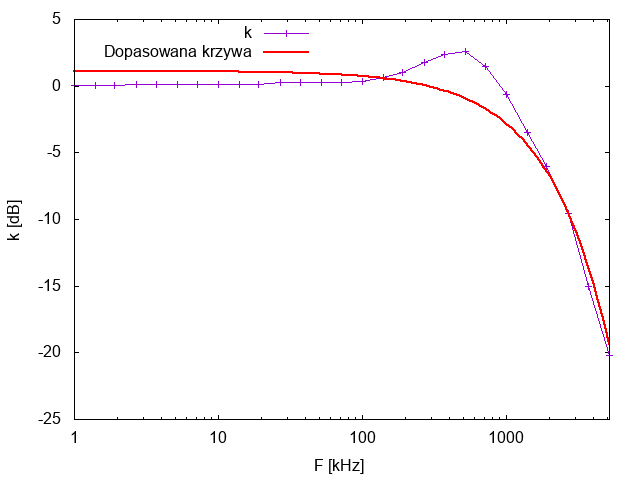
\includegraphics[width=7.5cm, height=6cm]{plot_wtornik_napieciowy_sin}
\caption{Wykres zależności wzmocnienia od częstotliwości w skali logarytmicznej.}
\end{figure}

\newpage

\subsubsection{Porównanie wzmocnień dla sygnału prostokątnego i sinusoidalnego}

Wzmocnienie dla sygnału prostokątnego wynosiło $0.98123171$, w przypadku sygnału sinusoidalnego po dokonaniu regresji liniowej otrzymaliśmy wartość równą $0.82293133$.

\newpage

\subsection{Wzmacniacz nieodwracający}

\subsubsection{Schemat wzmacniacza nieodwracającego}

\begin{figure}[h]
\centering
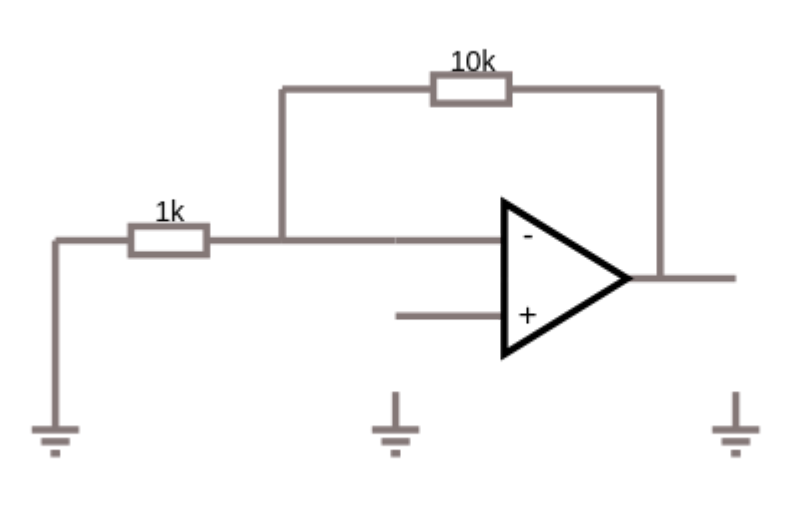
\includegraphics[width=10cm, height=6cm]{wno}
\caption{Schemat wzmacniacza nieodwracającego}
\end{figure}

\subsubsection{Zależność $U_{out}$ od $U_{in}$ oraz wzmocnienie}

\paragraph{Opór rezostora wynosi: $10\si{k\Omega}$}

\begin{figure}[h]
\centering
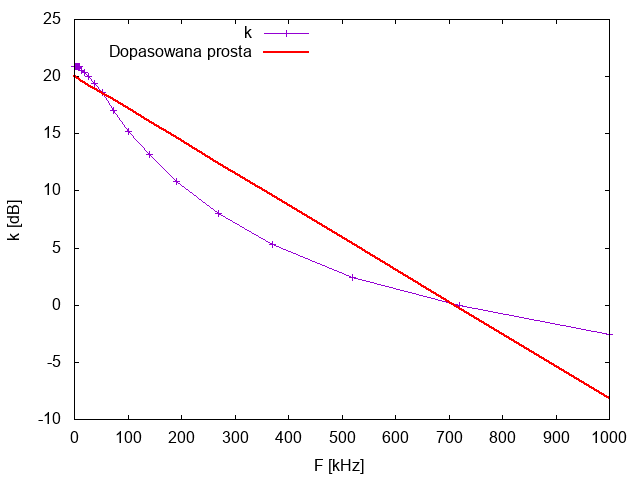
\includegraphics[width=7.5cm, height=6cm]{plot_nieodwracajacy_10kohm}
\caption{Wykres zależności wzmocnienia od częstotliwości w skali logarytmicznej.}
\end{figure}

\begin{center}
\begin{tabular}{ |p{3cm}|p{3cm}|p{3cm}|p{3cm}|p{3cm}| }
\hline
\makecell{Częstotliwość \\ $f$ [kHZ]} & \makecell{Wzmocnienie \\ $k$ [-]} & \makecell{Wzmocnienie \\ $k$ [dB]} & \makecell{Amplituda \\ wejścia [mV]} & \makecell{Amplituda \\ wyjścia [mV]} \\
\hline
0.1 & 11.05367302 & 20.87013227 & 101.075 & 1.11725 \\
0.14 & 11.02315161 & 20.84611561 & 100.425 & 1.107 \\
0.19 & 11.02315161 & 20.84611561 & 100.425 & 1.107 \\
0.27 & 11.02315161 & 20.84611561 & 100.425 & 1.107 \\
0.37 & 11.02315161 & 20.84611561 & 100.425 & 1.107 \\
0.52 & 11.02315161 & 20.84611561 & 100.425 & 1.107 \\
0.72 & 11.02315161 & 20.84611561 & 100.425 & 1.107 \\
1 & 11.02315161 & 20.84611561 & 100.425 & 1.107 \\
1.4 & 11.02315161 & 20.84611561 & 100.425 & 1.107 \\
1.9 & 11.02315161 & 20.84611561 & 100.425 & 1.107 \\
2.7 & 11.02315161 & 20.84611561 & 100.425 & 1.107 \\
3.7 & 11.02315161 & 20.84611561 & 100.425 & 1.107 \\
5.2 & 11.02315161 & 20.84611561 & 100.425 & 1.107 \\
7.2 & 11.02315161 & 20.84611561 & 100.425 & 1.107 \\
10 & 11.02315161 & 20.84611561 & 100.425 & 1.107 \\
14 & 10.65088757 & 20.54771601 & 101.4 & 1.08 \\
19 & 10.47199403 & 20.40058772 & 100.425 & 1.05165 \\
27 & 9.966962525 & 19.97125651 & 101.4 & 1.01065 \\
37 & 9.360453649 & 19.42593794 & 101.4 & 0.94915 \\
52 & 8.484148439 & 18.57216517 & 101.725 & 0.86305 \\
72 & 7.134922585 & 17.06778531 & 101.725 & 0.7258 \\
100 & 5.74522293 & 15.1861377 & 102.05 & 0.5863 \\
140 & 4.58010779 & 13.21751398 & 102.05 & 0.4674 \\
190 & 3.47121432 & 10.80962858 & 103.35 & 0.35875 \\
270 & 2.508684864 & 7.988922189 & 100.75 & 0.25275 \\
370 & 1.8358319 & 5.276658239 & 101.725 & 0.18675 \\
520 & 1.319734579 & 2.409731917 & 101.725 & 0.13425 \\
720 & 0.994311155 & -0.049553765 & 101.075 & 0.1005 \\
1000 & 0.74704142 & -2.533106356 & 101.4 & 0.07575 \\
\hline
\end{tabular}
\end{center}

\paragraph{Współczynnik wzmocnienia wynosi: -0.028153233 \\ Częstotliwość graniczna wynosi: $72kHz$}

\subsubsection{Zależność $U_{out}$ od $U_{in}$ oraz wzmocnienie}

\paragraph{Opór rezostora wynosi: $100\si{k\Omega}$}

\begin{figure}[h]
\centering
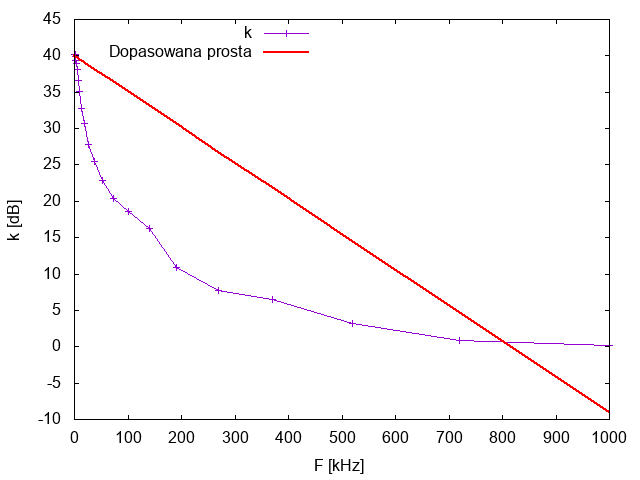
\includegraphics[width=7.5cm, height=6cm]{plot_nieodwracajacy_100kohm}
\caption{Wykres zależności wzmocnienia od częstotliwości w skali logarytmicznej.}
\end{figure}

\begin{center}
\begin{tabular}{ |p{3cm}|p{3cm}|p{3cm}|p{3cm}|p{3cm}| }
\hline
\makecell{Częstotliwość \\ $f$ [kHZ]} & \makecell{Wzmocnienie \\ $k$ [-]} & \makecell{Wzmocnienie \\ $k$ [dB]} & \makecell{Amplituda \\ wejścia [mV]} & \makecell{Amplituda \\ wyjścia [mV]} \\
\hline
0.1 & 101.4925373 & 40.1286822 & 20.1 & 2.04 \\
0.14 & 101.4925373 & 40.1286822 & 20.1 & 2.04 \\
0.19 & 101.4925373 & 40.1286822 & 20.1 & 2.04 \\
0.27 & 101.4925373 & 40.1286822 & 20.1 & 2.04 \\
0.37 & 101.4925373 & 40.1286822 & 20.1 & 2.04 \\
0.52 & 101.4925373 & 40.1286822 & 20.1 & 2.04 \\
0.72 & 101.4925373 & 40.1286822 & 20.1 & 2.04 \\
1 & 101.4925373 & 40.1286822 & 20.1 & 2.04 \\
1.4 & 101.4925373 & 40.1286822 & 20.1 & 2.04 \\
1.9 & 99.25373134 & 39.93493685 & 20.1 & 1.995 \\
2.7 & 93.03482587 & 39.37291098 & 20.1 & 1.87 \\
3.7 & 88.55721393 & 38.9444789 & 20.1 & 1.78 \\
5.2 & 80.59701493 & 38.12637914 & 20.1 & 1.62 \\
7.2 & 68.15920398 & 36.67049019 & 20.1 & 1.37 \\
10 & 56.55472637 & 35.04937811 & 20.1 & 1.13675 \\
14 & 43.28358209 & 32.7264639 & 20.1 & 0.87 \\
19 & 34.32835821 & 30.71306067 & 20.1 & 0.69 \\
27 & 24.62686567 & 27.82818283 & 20.1 & 0.495 \\
37 & 18.65671642 & 25.41670421 & 20.1 & 0.375 \\
52 & 13.93034826 & 22.87923948 & 20.1 & 0.28 \\
72 & 10.44776119 & 20.38046475 & 20.1 & 0.21 \\
100 & 8.457711443 & 18.54505728 & 20.1 & 0.17 \\
140 & 6.467661692 & 16.2149459 & 20.1 & 0.13 \\
190 & 3.529850746 & 10.95512685 & 20.1 & 0.07095 \\
270 & 2.43159204 & 7.71781426 & 20.1 & 0.048875 \\
370 & 2.114427861 & 6.503857453 & 20.1 & 0.0425 \\
520 & 1.437810945 & 3.154035707 & 20.1 & 0.0289 \\
720 & 1.099502488 & 0.823924325 & 20.1 & 0.0221 \\
1000 & 1.014925373 & 0.1286822 & 20.1 & 0.0204 \\
\hline
\end{tabular}
\end{center}

\paragraph{Współczynnik wzmocnienia wynosi: -0,049030086 \\ Częstotliwość graniczna wynosi: $85kHz$}

\subsection{Wzmacniacz logarytmiczny}

\subsubsection{Schemat wzmacniacza logarytmicznego}

\begin{figure}[h]
\centering
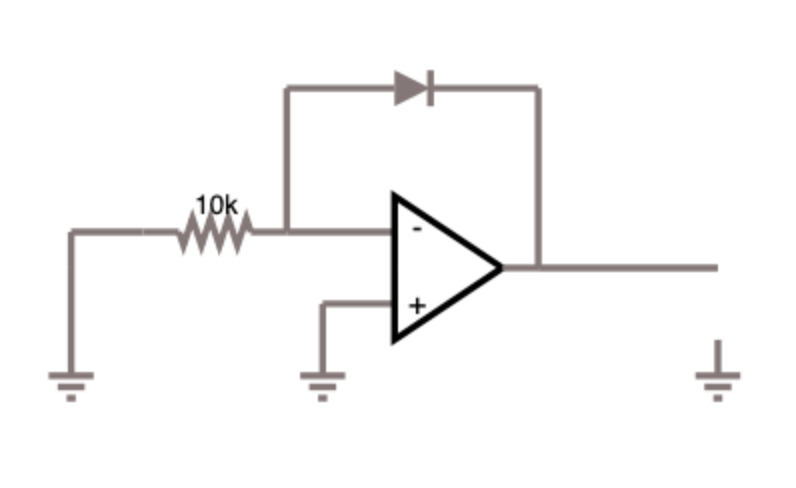
\includegraphics[width=10cm, height=6cm]{wl}
\caption{Schemat wzmacniacza logarytmicznego}
\end{figure}

\subsubsection{Zależność napięcia $V_{out}$ od napięcia $V_{in}$}

\begin{center}
\begin{tabular}{ |c|c| }
\hline
\makecell{Napięcie wejścia $V_{in}$ [mV]} & \makecell{Napięcie wyjścia $V_{out}$ [mV]} \\
\hline
10 & 304 \\
14 & 318 \\
19 & 330 \\
27 & 343 \\
37 & 355 \\
52 & 367 \\
72 & 379 \\
100 & 391 \\
140 & 404 \\
190 & 415.1 \\
270 & 428.2 \\
370 & 440 \\
520 & 453 \\
720 & 465 \\
1000 & 478 \\
1400 & 492.5 \\
1900 & 505 \\
2700 & 520 \\
3700 & 533 \\
5200 & 548 \\
7200 & 562 \\
10000 & 576 \\
\hline
\end{tabular}
\end{center}

\begin{figure}[h]
\centering
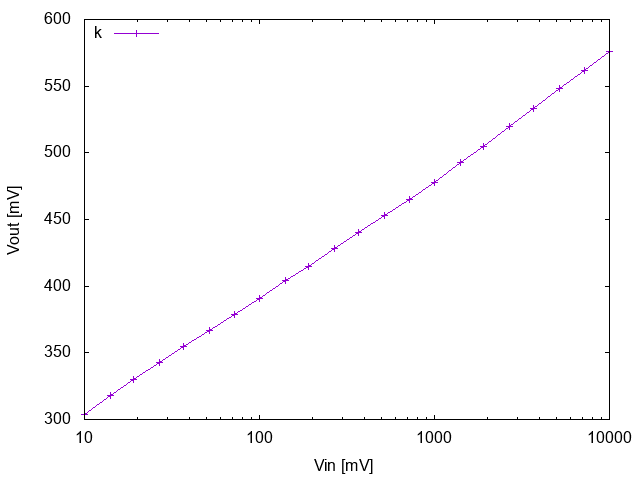
\includegraphics[width=7.5cm, height=6cm]{plot_logarytmiczny}
\caption{Wykres zależności napięcia $V_{out}$ od napięcia $V_{in}$ ($V_{in}$ w skali logarytmicznej).}
\end{figure}

\paragraph{\,}

\end{justify}
\end{document}